\section{Contexto de Negócio}
	A ESN é uma micro-empresa que atua na área de \textit{e-commerce} para pequenas empresas. Para apresentar destaque sobre os concorrentes, a ESN implementa técnicas de SEO, técnica que facilita o aparecimento de novos sites em motores de busca. Também é fornecida consultoria de publicidade aos clientes.

	A empresa se organiza em três áreas:
	\begin{itemize}
	{
		\item Grupo de Desenvolvimento;
		\item Grupo de \textit{Marketing};
		\item Grupo de Atendimento ao Cliente;
	}
	\end{itemize}

	Ao ser contratada, a ESN fornece um site simples e padronizado ao cliente disponibilizando o acesso ao painel de administração. Dessa forma, o cliente tem a possibilidade de realizar ações como inserir e editar categorias, programações, acessar relatórios e gerenciar pedidos. Também é fornecida a opção de customizar o layout através de templates.

	Atualmente, a ESN tem problemas na área referente à Pesquisa de Mercado da empresa. Existe uma dependência entre atividades que tem demandado muito tempo e dificultado o segmento processo. Além dessa dependência há a lentidão na realização da pesquisa já que a mesma é manual, ou seja, pessoas vão de porta em porta para realizar a pesquisa.

	\subsection{Descrição do Processo de Negócio Atual \textit{(AS-IS).}}

		Segundo Ferreira (2013), o fluxo de processo que determina exatamente onde as atividades de agregação de valor são realizadas atualmente no contexto da empresa é denominado \textit{AS-IS}.

		O processo de Planejamento de \textit{Marketing} a seguir foi modelado pela Equipe de Modelagem, e foram apresentados quatro sub-processos: Pesquisa de Mercado; Definição de Público-Alvo; Posicionamento do Produto; e, \textit{Marketing Mix}.

		A seguir estão contemplados os Planejamento de \textit{Marketing} desenvolvido atualmente pela empresa e o sub-processo de Pesquisa de Mercado, foco deste trabalho.

		\begin{figure}[!htp]
			\centering
			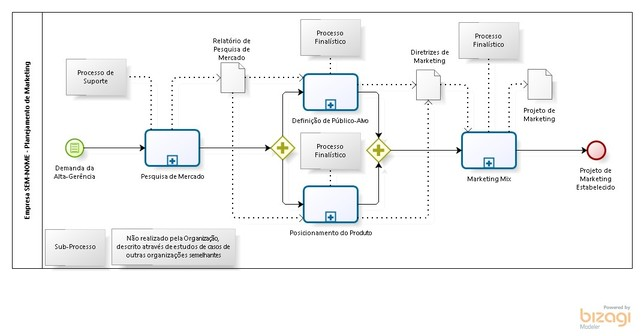
\includegraphics{imagens/as-is.jpg}
			\caption{Processo atual do planejamento de marketing da ESN.}
			\label{imagem}
		\end{figure}

		\newpage
		\vspace*{1cm}
		O processo de criação do Roteiro de Pesquisa é atualmente realizado de maneira lenta, pois uma atividade só pode ter início após a finalização por completo da atividade anterior. Um exemplo disso é o processo de validação do Roteiro de Pesquisa sendo iniciado apenas após o mesmo ser concluído.
		\begin{figure}[!htp]
			\centering
			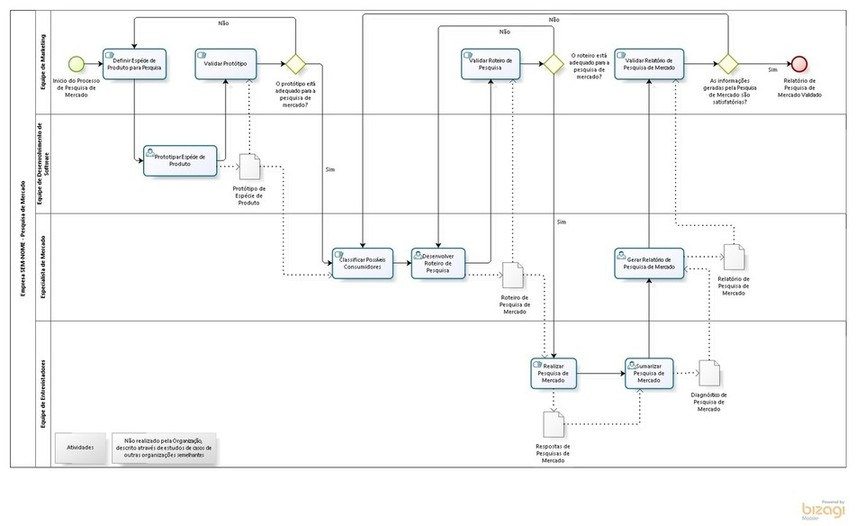
\includegraphics{imagens/as-is2.jpg}
			\caption{Processo atual da pesquisa de mercado da ESN.}
			\label{imagem}
		\end{figure}

		\newpage
	\subsection{Descrição do Processo de Negócio Futuro(\textit{TO-BE}).}

	De acordo com Ferreira (2013), o fluxo \textit{TO-BE} consiste na representação do processo a ser implementado ou proposição de um novo. Para este trabalho, a Equipe de Modelagem propôs um novo processo para a Pesquisa de Mercado da ESN.

	O fluxo a seguir foi identificado com a finalidade de representar o processo que será contemplado na aplicação a ser desenvolvida.

	Quatro papéis interagem com o processo de Pesquisa de Mercado, são eles: Equipe de Marketing, Equipe de Desenvolvimento de Software, Especialista de Mercado e Clientes Voluntários. O processo é iniciado quando ao surgir uma Necessidade de Pesquisa de Mercado a Equipe de Marketing define a espécie de Produto para a Pesquisa. Em seguida, três atividades são realizadas paralelamente. 

	O Especialista de Mercado classifica possíveis consumidores, a Equipe de Desenvolvimento de Software cria um protótipo para espécie de produto e a Equipe de Marketing valida o protótipo.

	Na próxima etapa do processo outras duas atividades são paralelizadas, o Especialista de Mercado é responsável por desenvolver o Roteiro de Pesquisa e a Equipe de Marketing por validá-lo. O Roteiro de Pesquisa é composto por diversos tópicos. Ao passo que o Especialista de Mercado vai criando cada tópico, os mesmos já chegam para a Equipe de Marketing para que a mesma possa validá-los. Dessa forma, o processo é agilizado.

	Após validado o Roteiro de Pesquisa, passa-se para a etapa de resposta de Pesquisa de Mercado realizada por Clientes Voluntários e gerenciada pela Equipe de Marketing. Caso as informações geradas pela Pesquisa de Mercado sejam satisfatórias o processo é finalizado, senão retorna-se para o início e é definida a Espécie de Produto para Pesquisa novamente.


	<Imagem>
